\documentclass[border=6pt]{standalone}

% tikz-style.tex (общий стиль для всех TikZ-картинок)
\RequirePackage[T1,T2A]{fontenc}
\RequirePackage[utf8]{inputenc}

% Palatino-подобный шрифт (как в MathJax часто воспринимается «более вытянутым»)
\RequirePackage{txfonts}
% txfonts даёт предупреждение по кириллице (T2A/txr не определён).
% Оставляем txfonts для математики, а текстовый шрифт возвращаем на Computer Modern,
% чтобы не искать T2A/txr и убрать предупреждения.
\renewcommand{\rmdefault}{cmr}
\renewcommand{\sfdefault}{cmss}
\renewcommand{\ttdefault}{cmtt}

\RequirePackage{tikz}
\RequirePackage{xcolor}
\usetikzlibrary{calc}

% цвета
\definecolor{lightgreen}{RGB}{214,234,214}
\definecolor{darkgreen}{HTML}{0B7A0B}
\definecolor{darkred}{HTML}{DF0000}

\definecolor{midgreen}{HTML}{2E9B2E}
\definecolor{palegreen}{RGB}{235,246,235}
\definecolor{olivegreen}{HTML}{3E6B2F}

\definecolor{lightred}{RGB}{255,220,220}
\definecolor{midred}{HTML}{E04545}
\definecolor{darkred2}{HTML}{A80000}

\definecolor{lightblue}{RGB}{220,232,255}
\definecolor{midblue}{HTML}{2E5BD6}
\definecolor{darkblue}{HTML}{0B2E8A}

\definecolor{lightgray}{RGB}{240,240,240}
\definecolor{midgray}{RGB}{170,170,170}
\definecolor{darkgray}{RGB}{80,80,80}

\definecolor{vtxfill}{RGB}{86,193,255}
\definecolor{vennfill}{RGB}{220,232,255}


% единый набор стилей TikZ
\tikzset{
    lab/.style={
        font=\fontsize{24}{32}\selectfont
    }
}

\usetikzlibrary{matrix,fit,calc}

\begin{document}
  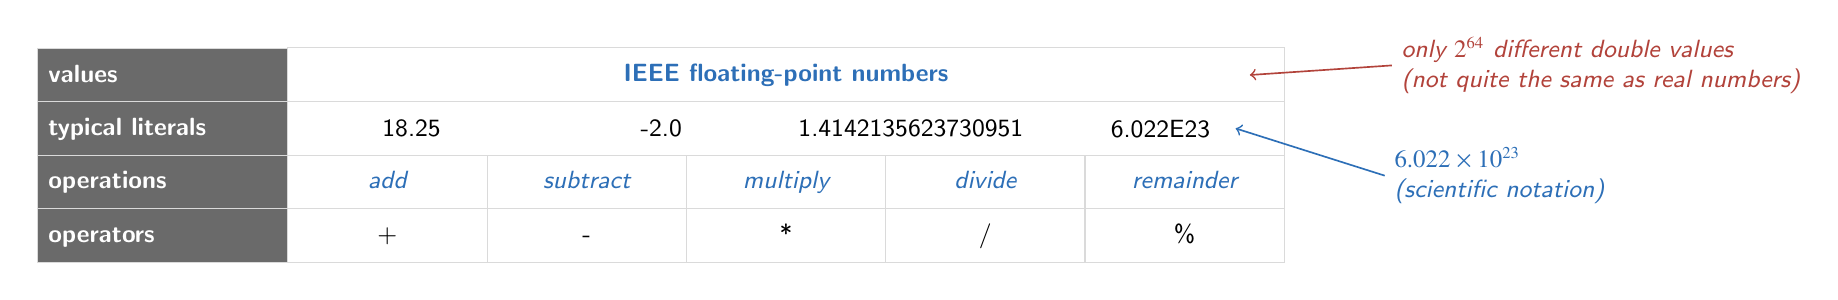
\begin{tikzpicture}
    \def\rowlabelw{2.9cm}
    \def\colw{2.35cm}
    \def\rowh{6.8mm}

    \definecolor{tbl-dark}{HTML}{6A6A6A}
    \definecolor{tbl-light}{HTML}{E6E6E6}
    \definecolor{tbl-border}{HTML}{DADADA}
    \definecolor{tbl-blue}{HTML}{2D6FB7}
    \definecolor{tbl-red}{HTML}{B2433B}

    \tikzset{
      tblcell/.style={
        draw=tbl-border,
        line width=0.35pt,
        minimum height=\rowh,
        text height=1.45ex,
        text depth=0.25ex,
        align=center,
        font=\sffamily\small,
        inner xsep=2.6pt,
        inner ysep=1.2pt
      },
      datacell/.style={
        tblcell,
        text width=\colw
      },
      headcell/.style={
        datacell,
        fill=white
      },
      rowlabel/.style={
        tblcell,
        fill=tbl-dark,
        text=white,
        font=\sffamily\bfseries\small,
        text width=\rowlabelw,
        align=left,
        inner xsep=4pt
      },
      opcell/.style={
        datacell,
        text=tbl-blue,
        font=\sffamily\itshape\small
      },
      ann/.style={
        font=\sffamily\itshape\small,
        align=left
      },
      annarrow/.style={
        ->,
        line width=0.6pt
      }
    }

    \matrix (tbl) [matrix of nodes, nodes in empty cells,
      nodes={datacell},
      row sep=-\pgflinewidth, column sep=-\pgflinewidth] {
      |[rowlabel]| values
      & |[headcell, draw=none]| & |[headcell, draw=none]| & |[headcell, draw=none]| & |[headcell, draw=none]| & |[headcell, draw=none]| \\
      |[rowlabel]| typical literals
      & |[draw=none]| & |[draw=none]| & |[draw=none]| & |[draw=none]| & |[draw=none]| \\
      |[rowlabel]| operations
      & |[opcell]| add & |[opcell]| subtract & |[opcell]| multiply & |[opcell]| divide & |[opcell]| remainder \\
      |[rowlabel]| operators
      & + & - & * & / & \% \\
    };

    \node[fit=(tbl-1-2)(tbl-1-6), draw=tbl-border, line width=0.35pt, fill=white, inner sep=0pt] (header) {};
    \node[font=\sffamily\bfseries\itshape\small, text=tbl-blue] at (header)
      {IEEE floating-point numbers};

    \node[fit=(tbl-2-2)(tbl-2-6), draw=tbl-border, line width=0.35pt, fill=white, inner sep=0pt] (row2box) {};
    \node[font=\sffamily\small] (lit1) at ($(row2box.west)!0.125!(row2box.east)$) {18.25};
    \node[font=\sffamily\small] (lit2) at ($(row2box.west)!0.375!(row2box.east)$) {-2.0};
    \node[font=\sffamily\small] (lit3) at ($(row2box.west)!0.625!(row2box.east)$) {1.4142135623730951};
    \node[font=\sffamily\small] (lit4) at ($(row2box.west)!0.875!(row2box.east)$) {6.022E23};

    \coordinate (headerpoint) at ($(header.east)+(-0.45cm,0)$);
    \node[ann, text=tbl-red, anchor=east] (noteA) at ($(tbl-2-5.east)+(+9.2cm,0.8cm)$) {only $2^{64}$ different double values\\(not quite the same as real numbers)};
    \draw[annarrow, tbl-red] (noteA.west) -- (headerpoint);

    \coordinate (numanchor) at ($(lit4.east)+(0.2cm,0)$);
    \node[ann, text=tbl-blue, anchor=west] (noteB) at ($(tbl-2-5.east)+(3.8cm,-0.6cm)$) {\(6.022 \times 10^{23}\)\\(scientific notation)};
    \draw[annarrow, tbl-blue] (noteB.west) -- (numanchor);
  \end{tikzpicture}
\end{document}
